\documentclass{standalone}
\usepackage{tikz}
\usepackage{float}
\usepackage{lmodern}
\usepackage{amsmath}
\usepackage{xcolor}
\usetikzlibrary{calc}
\usetikzlibrary{decorations.markings, decorations.pathreplacing}

\begin{document}

\centering

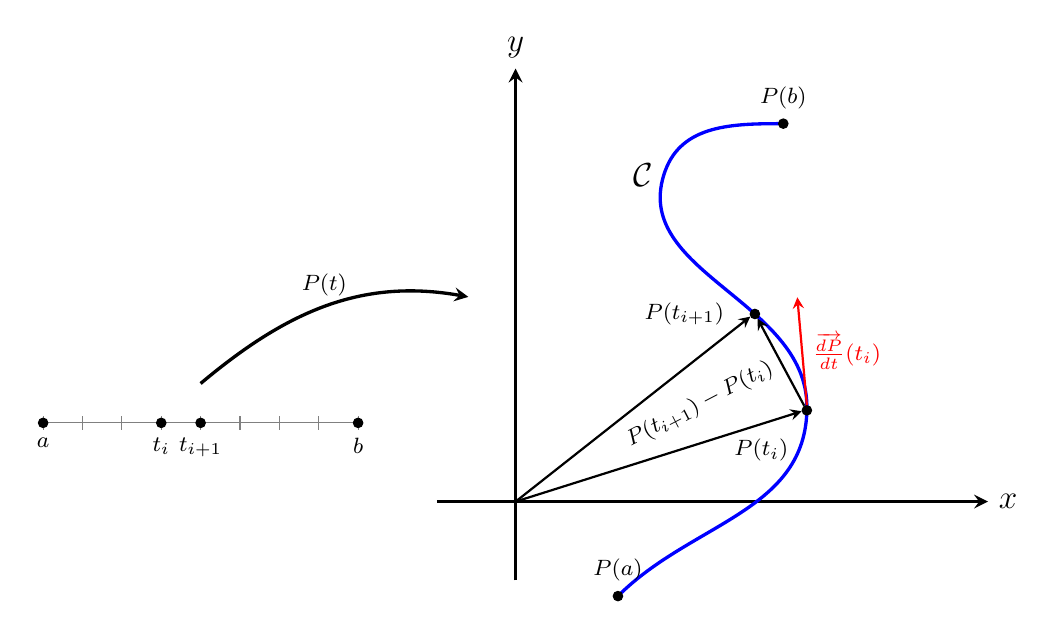
\begin{tikzpicture}[scale=1.0]
\pgfmathsetmacro{\CircleSize}{0.06}     % radius of coordinate circles/dots
% define styles used in this picture
\tikzset{
BigTextFont/.style={font=\large},   % Big text font
every node/.style={font=\footnotesize,text=black},  % Small text font
CircleNodeStyle/.style={draw=black, shape=circle, fill=black, minimum size=\CircleSize*2 cm, inner sep=0pt},
CircleStyle/.style={fill=black, radius=\CircleSize},
arrowstyle/.style={->, >=stealth}}

% custom colors
\definecolor{Red}{rgb}{1, 0, 0}
\definecolor{Blue}{rgb}{0, 0, 1}

% create axes
\pgfmathsetmacro{\OvershootAxis}{1.0}
\draw[arrowstyle, very thick] (-\OvershootAxis,0) -- (6,0) node[pos=1, right, BigTextFont] {$x$};
\draw[arrowstyle, very thick] (0,-\OvershootAxis) -- (0,5.5) node[pos=1, above, BigTextFont] {$y$};

\begin{scope}[xshift=-0.5cm]
    % defining the smooth curve (S-curve):
    \pgfmathsetmacro{\BeginSection}{2.4}    % BeginSection width
    \pgfmathsetmacro{\BeginDip}{2.4}        % BeginSection dip in height   
    \pgfmathsetmacro{\MiddleSectionWidth}{-1.8}
    \pgfmathsetmacro{\MiddleSectionHeight}{3.0}
    \pgfmathsetmacro{\EndSection}{1.5}     % EndSection width
    \pgfmathsetmacro{\EndDip}{0.6}          % EndSection dip in height 
    % define the waypoints of the smooth curve
    \coordinate (Begin) at (1.8, -1.2);
    \coordinate (BeginBend) at ($(Begin)+(\BeginSection, \BeginDip)$);
    \coordinate (EndBend) at ($(BeginBend) + (\MiddleSectionWidth, \MiddleSectionHeight)$);
    \coordinate (End) at ($(EndBend) + (\EndSection, \EndDip)$);
    % decorate the path with marks along the path
    \draw[postaction={decorate}, decoration={
        markings,
        mark=at position 0.80 with {\node[left, BigTextFont] {$\mathcal{C}$};},  % smooth curve symbol
        mark=at position 0.39 with \coordinate (Ti1);,       % T_(i) on smooth curve
        mark=at position 0.55 with \coordinate (Ti2);, }]    % T_(i+1) on smooth curve
    % draw the smooth curve
    [very thick, Blue] (Begin) to[out=45, in=180+90] (BeginBend) to[out=90, in=180+70] (EndBend) to[out=70, in=180] (End);
\end{scope}

% place domain range
\coordinate (BeginDomain) at (-2,1.0);
\pgfmathsetmacro{\WidthDomain}{4.0}
\coordinate (EndDomain) at ($(BeginDomain) + (-\WidthDomain, 0)$);
% thicks on domain range and place dots
\draw[postaction = {draw, decorate, decoration = {ticks, segment length=0.5cm}}]   % draw thicks on range
[gray] (BeginDomain) -- (EndDomain)
    node[pos=1, CircleNodeStyle, label=below:$a$] {}
    node[pos=0.625, CircleNodeStyle, label=below:$t_{i}$] {}
    node[pos=0.5, CircleNodeStyle, label=below:$t_{i+1}$] {}
    node[pos=0, CircleNodeStyle, label=below:$b$] {};

% P(t) transformation arrow
\draw[postaction={decorate}, decoration={
    markings,
    mark=at position 0.5 with {\node[above] {$P(t)$};}}]
[arrowstyle, very thick] ($(BeginDomain)!0.5!(EndDomain)+(0,0.5)$)  to[out=40,in=170] (-0.6,2.6);

% corresponding dots with label after transformation
\node [CircleNodeStyle, label=above:$P(a)$] at (Begin) {};
\node [CircleNodeStyle, label=above:$P(b)$] at (End) {};
\node [CircleNodeStyle, label={[label distance=0.2cm]245:$P(t_{i})$}] (Ti1Node) at (Ti1) {};
\node [CircleNodeStyle, label={[label distance=0.2cm]180:$P(t_{i+1})$}] (Ti2Node) at (Ti2) {};

% vectors
\draw[arrowstyle, thick] (0,0) -- (Ti1Node.190);
\draw[arrowstyle, thick] (Ti1Node.120) -- (Ti2Node.300)
    node[pos=0.5, left, rotate=27.5] at ($(Ti1)!0.5!(Ti2)$) {$P(t_{i+1})-P(t_{i})$};
\draw[arrowstyle, thick] (0,0) -- (Ti2Node.210);

% draw tangent
\coordinate (EndTangent) at ($(BeginBend) + (95:1.4)$);
\draw[arrowstyle, thick, Red] (Ti1Node.north) -- (EndTangent)
    node[pos=0.5, right, text=Red] {$\frac{\overrightarrow{dP}}{dt}(t_{i})$};

\end{tikzpicture}

\end{document}